\documentclass[11pt,a4paper]{article}
\usepackage[utf8]{inputenc}
\usepackage{amsmath}
\usepackage{amsfonts}
\usepackage{amssymb}
\usepackage{graphicx}
\author{Barbara Wiedermann}
\begin{document}
	\section{Kap. 1) Folgen und Reihen}
	\subsection{Grundidee}
	 	Baggersee 1500m\textsuperscript{2} Fläche er wird so ausgehoben, dass er jede Woche um 200m\textsuperscript{2} wächst Algen breiten sich aus.\\
	 	Am Beginn: 1m\textsuperscript{2} -\textgreater Verdreifacht sich wöchentlich\\
	 	
\begin{tabular}{|l|l|l|l|l|l|l|}
\hline
(n)Wochen    & 0    & 1    & 2    & 3    & 4...    & 8    \\ \hline
See Fläche   & 1500 & 1700 & 1900 & 2500 & 2300... & 3100 \\ \hline
Algen Fläche & 1    & 3    & 9    & 27   & 81...   & 6561 \\ \hline
\end{tabular}\\\\\\
Gesetz: Seefläche: 1500+200n\\
Algenfläche: /*3\textsuperscript{n}\\
n $\epsilon$ $\mathbb{N}$ \textsubscript{0} \\

Definition: Eine Folge ist eine Abbildung: \\
f: $\mathbb{N}$ -$>$ $\mathbb{R}$ bzw. f: $\mathbb{N}$ -$>$ $\mathbb{C}$\\
($\mathbb{N}$ manchmal)\\

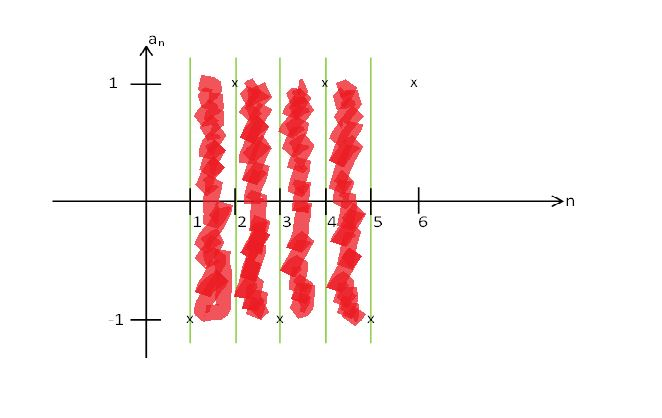
\includegraphics[width = 0.7\textwidth]{img/Zeichnung.jpg}

\end{document}